\documentclass[border=0.2cm]{standalone}
% \usepackage{emoji}
\usepackage{DejaVuSans}
\usepackage{tikz}
\usetikzlibrary{positioning,automata,backgrounds}

\tikzset{>=latex} % for LaTeX arrow head
\usepackage{xcolor}

% taken from neural networks
\usepackage{amsmath} % for aligned
%\usepackage{amssymb} % for \mathbb
%\usepackage{etoolbox} % for \ifthen
\usepackage{listofitems} % for \readlist to create arrays
\usetikzlibrary{arrows.meta} % for arrow size
\usepackage[outline]{contour} % glow around text
\contourlength{1.4pt}


% to draw hulls between groups of nodes
% taken from 
% https://tex.stackexchange.com/questions/70999/highlight-a-group-of-nodes-in-a-tikz-tree
\pgfdeclarelayer{background}
\pgfsetlayers{background,main}
\newcommand{\convexpath}[2]{
[   
    create hullnodes/.code={
        \global\edef\namelist{#1}
        \foreach [count=\counter] \nodename in \namelist {
            \global\edef\numberofnodes{\counter}
            \node at (\nodename) [draw=none,name=hullnode\counter] {};
        }
        \node at (hullnode\numberofnodes) [name=hullnode0,draw=none] {};
        \pgfmathtruncatemacro\lastnumber{\numberofnodes+1}
        \node at (hullnode1) [name=hullnode\lastnumber,draw=none] {};
    },
    create hullnodes
]
($(hullnode1)!#2!-90:(hullnode0)$)
\foreach [
    evaluate=\currentnode as \previousnode using \currentnode-1,
    evaluate=\currentnode as \nextnode using \currentnode+1
    ] \currentnode in {1,...,\numberofnodes} {
  let
    \p1 = ($(hullnode\currentnode)!#2!-90:(hullnode\previousnode)$),
    \p2 = ($(hullnode\currentnode)!#2!90:(hullnode\nextnode)$),
    \p3 = ($(\p1) - (hullnode\currentnode)$),
    \n1 = {atan2(\y3,\x3)},
    \p4 = ($(\p2) - (hullnode\currentnode)$),
    \n2 = {atan2(\y4,\x4)},
    \n{delta} = {-Mod(\n1-\n2,360)}
  in 
    {-- (\p1) arc[start angle=\n1, delta angle=\n{delta}, radius=#2] -- (\p2)}
}
-- cycle
}

% using tableau 10 color palette: https://public.tableau.com/views/TableauColors/ColorPaletteswithRGBValues?%3Aembed=y&%3AshowVizHome=no&%3Adisplay_count=y&%3Adisplay_static_image=y

\definecolor{myblue}{RGB}{31,119,180}
\definecolor{myred}{RGB}{214,39,40}
\definecolor{mygreen}{RGB}{44,160,44}
\definecolor{myorange}{RGB}{255,127,14}

\colorlet{mydarkred}{red!30!black}
\colorlet{mydarkblue}{blue!40!black}
\colorlet{mydarkgreen}{green!30!black}
\tikzstyle{node}=[ultra thick,circle,minimum size=30,inner sep=2.,outer sep=0.6]
\tikzstyle{node green}=[node,fill=mygreen]
\tikzstyle{node blue}=[node,fill=myblue]
\tikzstyle{node orange}=[node,orange!20!black,draw=myorange!30!black,fill=myorange!20]
\tikzstyle{node red}=[node,fill=myred]
\tikzstyle{connect}=[very thick,mydarkblue] %,line cap=round
\tikzstyle{connect arrow}=[-{Latex[length=4,width=3.5]},very thick,mydarkblue,shorten <=0.5,shorten >=1, <->]
\tikzset{ % node styles, numbered for easy mapping with \nstyle
  node 1/.style={node in},
  node 2/.style={node hidden},
  node 3/.style={node out},
}
\def\nstyle{int(\lay<\Nnodlen?min(2,\lay):3)} % map layer number onto 1, 2, or 3
 

% spacing nodes
% \tikzset{node distance = 0.5cm and 0.5cm}

\begin{document}
 
\begin{tikzpicture}[
    node distance=3cm,
    on grid,
    very thick,
    font=\large
    ]
 
% % Mode 1    
% \node at (-1.5,0.5) (q_fr)
% {
%     
\includegraphics[height=1.3cm]{france.png}
% };
\node at (-0.1,-2) (q_fr) [opacity=0.3]
{
    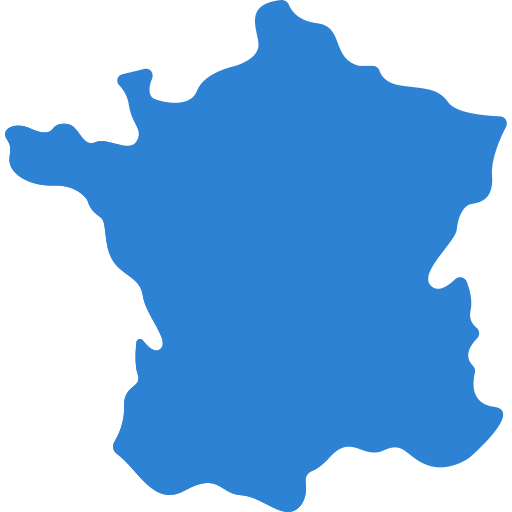
\includegraphics[height=7cm]{france-3.png}
};

% Mode 1    
\node [node] (q_0)
{
    
\includegraphics[width=1cm]{car.png}
};
 
% Mode 2    
\node [node] (q_1) [below right=of q_0]
{
    
\includegraphics[width=1cm]{jerrycan.png}
};

% Mode 2, to nicely place the rectangle   
\node [node] (q_3) [below left=of q_0]
{
};


% Mode 3    
\node [node] (q_2) [below left=of q_1]
{
    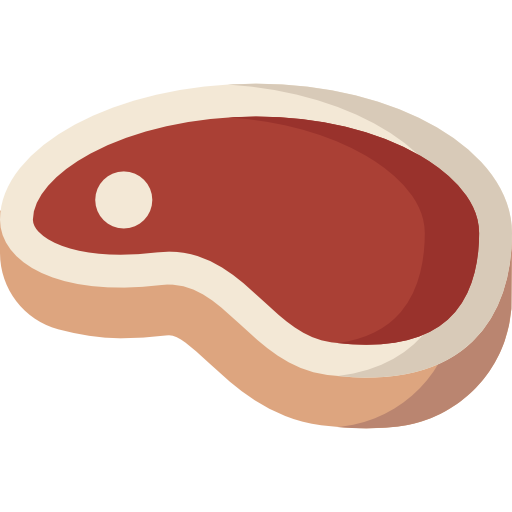
\includegraphics[width=1cm]{meat.png}
};

\node (q_w) [right=5cm of q_1, opacity=0.3]
{
    
\includegraphics[height=4cm]{worldwide.png}
};

% Mode 2 bar
\node [node] (q_1_bar) [right=4cm of q_1]
{
    
\includegraphics[width=1cm]{jerrycan.png}
};

% Mode 1 bar 
\node [ node] (q_0_bar) [above right=1.5cm of q_1_bar]
{
    
\includegraphics[width=1cm]{car.png}
};
 
% Mode 3    
\node [node] (q_2_bar) [below right=1.5cm of q_1_bar]
{
    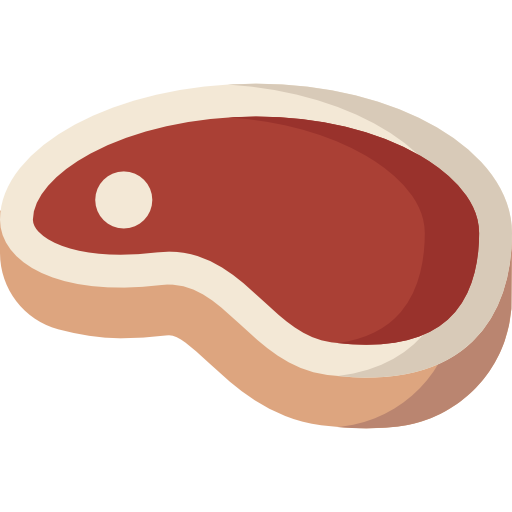
\includegraphics[width=1cm]{meat.png}
};

% % Mode 1    
% \node [node] (q_w) [above=2cm of q_0_bar]
% {
%     World \raisebox{-0.4\height}{
\includegraphics[height=1cm]{worldwide.png}}
% };

% Mode 2, to nicely place the rectangle   
\node [node] (q_3_bar) [below right=of q_0_bar]
{
};
 
% r_i
% \path [-latex] (q_0) edge [in=130,out=160,loop] node [above right] {$r_i$} (q_0);
% \path [-latex] (q_1) edge [in=30,out=60,loop] (q_1);
% \path [-latex] (q_2) edge [in=230,out=260,loop] (q_2);
% \path [-latex] (q_0_bar) edge [in=30,out=60,loop] (q_0_bar);
% \path [-latex] (q_1_bar) edge [in=130,out=160,loop]  (q_1_bar);
% \path [-latex] (q_2_bar) edge [in=-30,out=-60,loop] (q_2_bar);

% mu
\path [-latex] (q_0) edge [bend left=45, dashed, <->, myorange] 
    % node[right=0.5cm,fill=black!5,rounded corners]{
    % \begin{tabular}{c}
    %     Transfers\\
    %     $\mu$
    % \end{tabular}
    % } 
    (q_1);
\path [-latex] (q_1) edge [bend left=45, dashed, <->, myorange] (q_2);
\path [-latex] (q_2) edge [bend left=45, dashed, <->, myorange] (q_0);

% \path [-latex] (q_0_bar) edge [bend right=45, dashed, <->, myblue!50] (q_1_bar);
% \path [-latex] (q_1_bar) edge [bend right=45, dashed, <->, myblue!50] (q_2_bar);
% \path [-latex] (q_2_bar) edge [bend right=45, dashed, <->, myblue!50] (q_0_bar);

% DELTA
\path [-latex] (q_0) edge [dashed, <->, very thick, mygreen, bend left=20] 
%      node [above=0.5cm,fill=black!5,rounded corners] {
%     \begin{tabular}{c}
%         Spatial transfers\\
%         $\delta$
%     \end{tabular}
%     } 
(q_0_bar);
\path [-latex] (q_1) edge [dashed, <->, very thick, mygreen] (q_1_bar);
\path [-latex] (q_2) edge [dashed, <->, very thick, mygreen, bend right=20] (q_2_bar);


% ALPHA
\begin{scope} [connect arrow]  % now dashed is for the lines inside the scope
    \draw (q_0) -- (q_1)  ; 
    \draw (q_1) -- (q_2)  ; 
    \draw (q_2) --
        %  node[left=0.2cm,fill=black!5,rounded corners]{
        % \begin{tabular}{c}
        %     Interactions\\
        %     $\alpha$
        % \end{tabular}
        % }
        (q_0)  ; 
    % \draw (q_0_bar) -- (q_1_bar)  ; 
    % \draw (q_2_bar) -- (q_0_bar)  ; 
    % \draw (q_1_bar) -- (q_2_bar)  ; 
\end{scope}

\draw[connect arrow] (q_0) -- (q_1);

% \begin{pgfonlayer}{background}
%     \filldraw [line width=4mm,join=round,black!10]
%       (q_0.north  -| q_1.east)  rectangle (q_2.south  -| q_3.center);
%     %   (q_w.north -| q_1_bar.west) rectangle (q_2_bar.south -| q_3_bar.center);
%   \end{pgfonlayer}

% Legend
\path ([xshift=-2cm,yshift=1.5cm]current bounding box.north)
node[matrix,anchor=north west,cells={nodes={font=\sffamily,anchor=west}},thick,inner sep=1ex]{
 \draw[connect arrow](0,0) -- ++ (1,0); & \node{Interactions, $\alpha$};\\
 \draw[-latex, dashed, <->, myorange](0,0) -- ++ (1.0,0); & \node{Transformations into other economic activities, $\mu$};\\
 \draw[dashed, <->, very thick, mygreen](0,0) -- ++ (1.,0); & \node{Spatial dispersal, $\delta$};\\
};

\end{tikzpicture}
 
\end{document}